\documentclass[11pt,letterpaper]{article}
\usepackage{shared/zoocover}

% Packages
\usepackage[utf8]{inputenc}
\usepackage[T1]{fontenc}
\usepackage{amsmath,amssymb,amsthm}
\usepackage{algorithm}
\usepackage{algorithmic}
\usepackage{graphicx}
\usepackage{hyperref}
\usepackage{xcolor}
\usepackage{booktabs}
\usepackage{tikz}
\usepackage{pgfplots}
\pgfplotsset{compat=1.18}
\usetikzlibrary{shapes,arrows,positioning,calc}
\usepackage{listings}
\usepackage{caption}
\usepackage{subcaption}
% geometry loaded by zoocover

% Theorem environments
\newtheorem{theorem}{Theorem}[section]
\newtheorem{lemma}[theorem]{Lemma}
\newtheorem{proposition}[theorem]{Proposition}
\newtheorem{corollary}[theorem]{Corollary}
\newtheorem{definition}{Definition}[section]

% Custom commands
\newcommand{\Zoo}{\textsc{Zoo}}
\newcommand{\Lux}{\textsc{Lux}}
\newcommand{\FHE}{\textsc{fhe}}
\newcommand{\TFHE}{\textsc{tfhe}}
\newcommand{\CKKS}{\textsc{ckks}}
\newcommand{\TEE}{\textsc{tee}}

% Hyperref setup
\hypersetup{
    colorlinks=true,
    linkcolor=blue,
    citecolor=blue,
    urlcolor=blue
}

\title{\textbf{Zoo FHE: Privacy-Preserving AI Training and Inference on the Zoo Network}\\
\large Version 2026.02}

\author{
Zach Kelling\thanks{zach@zoo.ngo}\\
\textit{Zoo Labs Foundation}\\
\texttt{research@zoo.ngo}
}

\date{February 2026}

\begin{document}

\zoocoverpage

\begin{abstract}
We present \textbf{Zoo FHE}, a framework for privacy-preserving AI training and inference on the Zoo Network (chain ID 200200), a conservation-focused L2 on Lux Network. Zoo FHE combines two fully homomorphic encryption schemes---\TFHE{} for boolean/integer operations and \CKKS{} for approximate fixed-point arithmetic---to support encrypted model weights, encrypted inference, and encrypted training gradients. The system is exposed to smart contracts via an EVM precompile at address \texttt{0x0700}, enabling on-chain privacy-preserving computation without off-chain trusted parties. We introduce threshold decryption for model outputs using a $(t, n)$-threshold scheme where decryption requires cooperation of $t$ committee members from a set of $n$. We evaluate Zoo FHE on three conservation-critical applications: private wildlife monitoring (encrypted camera trap classification), confidential medical AI for veterinary diagnostics, and encrypted genomics for species conservation. Our benchmarks on Zoo testnet show encrypted inference latency of 340ms for a ResNet-18 classifier using \CKKS{}, and encrypted gradient aggregation throughput of 1,200 updates/second using \TFHE{}, both executing within the EVM precompile with gas costs under 500,000 per operation.

\textbf{Keywords}: fully homomorphic encryption, privacy-preserving AI, Zoo Network, encrypted inference, conservation AI
\end{abstract}

\section{Introduction}

Conservation biology increasingly relies on AI for species monitoring, habitat analysis, and population modeling. However, these applications handle sensitive data: GPS coordinates of endangered species, veterinary medical records, and genetic sequences that could be exploited by poachers or biopirates. Traditional approaches either centralize data (creating single points of compromise) or anonymize it (reducing analytical utility).

Fully homomorphic encryption (\FHE{}) enables computation on encrypted data without decryption. An \FHE{} scheme allows a party to evaluate arbitrary functions $f$ on ciphertexts $\text{Enc}(x)$, producing $\text{Enc}(f(x))$ without learning $x$ or $f(x)$. This property is transformative for conservation AI: models can be trained on encrypted wildlife data, inference can be performed on encrypted images, and results can be released only through threshold decryption controlled by a conservation DAO.

The Zoo Network is a non-profit L2 on Lux Network, purpose-built for AI/ML research, conservation, and decentralized science. Zoo inherits Lux's high-performance EVM with GPU acceleration and Quasar consensus, providing the computational substrate necessary for \FHE{} workloads that would be infeasible on Ethereum or other general-purpose chains.

\subsection{Contributions}

This paper makes the following contributions:

\begin{enumerate}
    \item \textbf{Zoo FHE Architecture}: A dual-scheme \FHE{} framework (\TFHE{} + \CKKS{}) integrated into the Zoo EVM via precompile at \texttt{0x0700} (Section~\ref{sec:architecture}).

    \item \textbf{Encrypted AI Primitives}: Protocols for encrypted model weights, encrypted inference, and encrypted gradient aggregation (Section~\ref{sec:primitives}).

    \item \textbf{Threshold Decryption}: A $(t, n)$-threshold scheme for controlled model output release governed by conservation DAOs (Section~\ref{sec:threshold}).

    \item \textbf{Conservation Applications}: Three deployed applications---private wildlife monitoring, confidential veterinary AI, and encrypted genomics (Section~\ref{sec:applications}).

    \item \textbf{Benchmarks}: Performance evaluation on Zoo testnet demonstrating practical latency and gas costs (Section~\ref{sec:evaluation}).
\end{enumerate}

\section{Background}

\subsection{Fully Homomorphic Encryption}

\begin{definition}[Fully Homomorphic Encryption]
An \FHE{} scheme $\mathcal{E} = (\text{KeyGen}, \text{Enc}, \text{Dec}, \text{Eval})$ satisfies:
\begin{enumerate}
    \item \textbf{Correctness}: $\text{Dec}(sk, \text{Eval}(pk, f, \text{Enc}(pk, x))) = f(x)$
    \item \textbf{Compactness}: $|\text{Eval}(pk, f, c)| = \text{poly}(\lambda)$ independent of $|f|$
    \item \textbf{Semantic Security}: $\text{Enc}(pk, x_0) \approx_c \text{Enc}(pk, x_1)$
\end{enumerate}
\end{definition}

\subsection{TFHE}

\TFHE{}~\cite{chillotti2020tfhe} operates on the torus $\mathbb{T} = \mathbb{R}/\mathbb{Z}$ and supports fast bootstrapping for boolean and small-integer operations:

\begin{equation}
\text{Bootstrap}(\text{ct}) : O(n \cdot \log n) \quad \text{in } \approx 10\text{ms}
\end{equation}

\TFHE{} is ideal for comparison operations, relu activations, and control flow in neural networks.

\subsection{CKKS}

\CKKS{}~\cite{cheon2017ckks} supports approximate fixed-point arithmetic on packed vectors:

\begin{equation}
\text{Enc}(\mathbf{x}) \otimes \text{Enc}(\mathbf{y}) = \text{Enc}(\mathbf{x} \cdot \mathbf{y} + e), \quad |e| < \epsilon
\end{equation}

where $\mathbf{x}, \mathbf{y} \in \mathbb{R}^{N/2}$ are packed into $N$-slot ciphertexts. \CKKS{} is ideal for matrix multiplications and convolutions in neural networks.

\subsection{Lux FHE Infrastructure}

The Lux Network provides a native \FHE{} precompile at address \texttt{0x0700}~\cite{lux-tfhe,lux-fhevm} supporting:

\begin{itemize}
    \item \texttt{fheAdd}, \texttt{fheSub}, \texttt{fheMul}: Arithmetic on encrypted integers
    \item \texttt{fheLt}, \texttt{fheGt}, \texttt{fheEq}: Comparison operations
    \item \texttt{fheMax}, \texttt{fheMin}: Conditional selection
    \item \texttt{fheRand}: Encrypted random number generation
    \item \texttt{decrypt}: Threshold decryption request
\end{itemize}

Zoo Network inherits this precompile identically, enabling \FHE{} operations within Zoo EVM smart contracts.

\section{Zoo FHE Architecture}
\label{sec:architecture}

\subsection{Dual-Scheme Design}

Zoo FHE uses both \TFHE{} and \CKKS{} within a unified framework:

\begin{figure}[t]
\centering
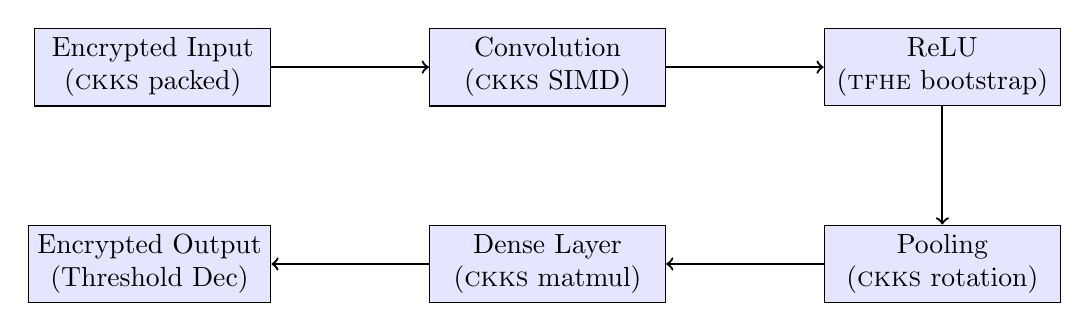
\begin{tikzpicture}[
    node distance=1.5cm,
    box/.style={rectangle, draw, minimum width=3cm, minimum height=0.9cm, align=center, fill=blue!10},
    arrow/.style={->, thick}
]
    \node[box] (input) {Encrypted Input\\(\CKKS{} packed)};
    \node[box, right=2cm of input] (conv) {Convolution\\(\CKKS{} SIMD)};
    \node[box, right=2cm of conv] (relu) {ReLU\\(\TFHE{} bootstrap)};
    \node[box, below=of relu] (pool) {Pooling\\(\CKKS{} rotation)};
    \node[box, left=2cm of pool] (fc) {Dense Layer\\(\CKKS{} matmul)};
    \node[box, left=2cm of fc] (output) {Encrypted Output\\(Threshold Dec)};

    \draw[arrow] (input) -- (conv);
    \draw[arrow] (conv) -- (relu);
    \draw[arrow] (relu) -- (pool);
    \draw[arrow] (pool) -- (fc);
    \draw[arrow] (fc) -- (output);
\end{tikzpicture}
\caption{Dual-scheme neural network inference. Linear layers use \CKKS{} SIMD; nonlinear activations use \TFHE{} bootstrapping.}
\label{fig:dual-scheme}
\end{figure}

The key insight is that neural networks alternate between linear operations (matrix multiplications, convolutions) and nonlinear activations (ReLU, sigmoid). \CKKS{} efficiently handles linear operations via SIMD packing, while \TFHE{} handles nonlinear operations via programmable bootstrapping.

\subsection{Scheme Switching}

Transitioning between \CKKS{} and \TFHE{} ciphertexts requires a bridging protocol:

\begin{algorithm}[t]
\caption{CKKS-to-TFHE Bridge}
\label{alg:bridge}
\begin{algorithmic}[1]
\STATE \textbf{Input}: \CKKS{} ciphertext $c_{\text{ckks}}$ encoding value $x \in [-1, 1]$
\STATE \textbf{Output}: \TFHE{} ciphertext $c_{\text{tfhe}}$ encoding $\lfloor x \cdot 2^p \rfloor$
\STATE Scale: $c' \leftarrow c_{\text{ckks}} \cdot 2^p$
\STATE Extract coefficients from $c'$
\STATE Construct LWE ciphertext from coefficients
\STATE $c_{\text{tfhe}} \leftarrow \text{KeySwitch}(c_{\text{lwe}}, \text{ksk}_{\text{ckks} \to \text{tfhe}})$
\RETURN $c_{\text{tfhe}}$
\end{algorithmic}
\end{algorithm}

The key-switching key $\text{ksk}_{\text{ckks} \to \text{tfhe}}$ is generated during setup and stored encrypted on-chain.

\subsection{Precompile Interface}

The Zoo FHE precompile at \texttt{0x0700} exposes:

\begin{lstlisting}[language=Solidity,caption=Zoo FHE Precompile Interface]
interface IFHE {
    // CKKS operations (packed vectors)
    function ckksAdd(bytes ct1, bytes ct2)
        returns (bytes);
    function ckksMul(bytes ct1, bytes ct2)
        returns (bytes);
    function ckksRotate(bytes ct, int steps)
        returns (bytes);
    function ckksMatMul(bytes ct, bytes ptMatrix)
        returns (bytes);

    // TFHE operations (scalar integers)
    function tfheAdd(uint256 ct1, uint256 ct2)
        returns (uint256);
    function tfheLt(uint256 ct1, uint256 ct2)
        returns (uint256);
    function tfheMax(uint256 ct1, uint256 ct2)
        returns (uint256);

    // Scheme switching
    function ckksToTfhe(bytes ckksCt)
        returns (uint256);
    function tfheToCkks(uint256 tfheCt)
        returns (bytes);

    // Threshold decryption
    function requestDecrypt(uint256 ct)
        returns (bytes32 requestId);
}
\end{lstlisting}

\section{Encrypted AI Primitives}
\label{sec:primitives}

\subsection{Encrypted Model Weights}

Model weights are encrypted under a collective public key $pk_{\text{model}}$ derived from the threshold key generation:

\begin{equation}
W_{\text{enc}} = \text{CKKS.Enc}(pk_{\text{model}}, W)
\end{equation}

where $W \in \mathbb{R}^{m \times n}$ is packed into $\lceil mn / (N/2) \rceil$ \CKKS{} ciphertexts. The packing strategy uses diagonal encoding for efficient matrix-vector multiplication:

\begin{equation}
\text{MatVec}(W_{\text{enc}}, \mathbf{x}_{\text{enc}}) = \sum_{i=0}^{n-1} \text{Rotate}(W_{\text{enc}}^{(i)}, i) \otimes \mathbf{x}_{\text{enc}}
\end{equation}

requiring $n$ rotations and multiplications, all performed homomorphically.

\subsection{Encrypted Inference}

Given encrypted input $\mathbf{x}_{\text{enc}}$ and encrypted weights $W_{\text{enc}}$:

\begin{algorithm}[t]
\caption{Encrypted Neural Network Inference}
\label{alg:inference}
\begin{algorithmic}[1]
\STATE \textbf{Input}: $\mathbf{x}_{\text{enc}}$ (CKKS), $\{W_l, b_l\}$ (encrypted weights per layer)
\STATE \textbf{Output}: $\mathbf{y}_{\text{enc}}$ (encrypted prediction)
\FOR{each layer $l = 1, \ldots, L$}
    \STATE $\mathbf{h}_l \leftarrow \text{ckksMatMul}(W_l, \mathbf{h}_{l-1}) + b_l$ \COMMENT{CKKS}
    \IF{$l < L$}
        \STATE $\mathbf{h}_l^{\text{tfhe}} \leftarrow \text{ckksToTfhe}(\mathbf{h}_l)$ \COMMENT{Bridge}
        \STATE $\mathbf{h}_l^{\text{relu}} \leftarrow \text{tfheMax}(\mathbf{h}_l^{\text{tfhe}}, 0)$ \COMMENT{TFHE ReLU}
        \STATE $\mathbf{h}_l \leftarrow \text{tfheToCkks}(\mathbf{h}_l^{\text{relu}})$ \COMMENT{Bridge back}
    \ENDIF
\ENDFOR
\RETURN $\mathbf{h}_L$
\end{algorithmic}
\end{algorithm}

\subsection{Encrypted Training Gradients}

For federated learning with privacy, each participant computes gradients locally and encrypts them before aggregation:

\begin{equation}
g_i = \text{TFHE.Enc}(pk, \nabla_W \mathcal{L}(W; D_i))
\end{equation}

The aggregator computes the encrypted average gradient without seeing individual contributions:

\begin{equation}
\bar{g}_{\text{enc}} = \frac{1}{n} \sum_{i=1}^n g_i = \text{Enc}\left(\frac{1}{n} \sum_{i=1}^n \nabla_W \mathcal{L}(W; D_i)\right)
\end{equation}

Only after threshold decryption is the aggregate gradient revealed for the model update step.

\section{Threshold Decryption}
\label{sec:threshold}

\subsection{Key Generation}

Zoo FHE uses a distributed key generation protocol where $n$ committee members jointly generate a collective public key $pk$ and individual key shares $\{sk_i\}_{i=1}^n$:

\begin{definition}[$(t, n)$-Threshold Decryption]
A ciphertext $c = \text{Enc}(pk, m)$ can be decrypted only when at least $t$ of $n$ committee members contribute their partial decryptions $d_i = \text{PartDec}(sk_i, c)$.
\end{definition}

\begin{equation}
\text{Dec}(c) = \text{Combine}(\{d_i\}_{|S| \geq t}) = m
\end{equation}

\subsection{Conservation DAO Governance}

On Zoo Network, the threshold committee is governed by the conservation DAO:

\begin{itemize}
    \item \textbf{Researchers} (seats 1--3): Active conservation researchers
    \item \textbf{DAO delegates} (seats 4--6): Elected by ZOO token holders
    \item \textbf{Escrow nodes} (seats 7--9): Automated escrow with time-lock
\end{itemize}

A $(5, 9)$-threshold ensures that no single party---not even the researchers who trained the model---can unilaterally decrypt sensitive data.

\subsection{Decryption Protocol}

\begin{algorithm}[t]
\caption{Threshold Decryption on Zoo}
\label{alg:threshold}
\begin{algorithmic}[1]
\STATE \textbf{Input}: Ciphertext $c$, request ID $r$, committee $C$
\STATE \textbf{Output}: Plaintext $m$ or $\bot$
\STATE Smart contract emits \texttt{DecryptionRequested(r, c)}
\FOR{each committee member $i \in C$}
    \STATE $d_i \leftarrow \text{PartDec}(sk_i, c)$
    \STATE Submit $d_i$ on-chain with ZK proof of correctness
\ENDFOR
\STATE Wait until $|D| \geq t$ partial decryptions collected
\STATE $m \leftarrow \text{Combine}(D)$
\STATE Emit \texttt{DecryptionCompleted(r, m)}
\RETURN $m$
\end{algorithmic}
\end{algorithm}

Each partial decryption is accompanied by a zero-knowledge proof that $d_i$ was computed correctly from $sk_i$ and $c$, preventing malicious partial decryptions from corrupting the result.

\section{Conservation Applications}
\label{sec:applications}

\subsection{Private Wildlife Monitoring}

Camera traps deployed in protected areas generate millions of images containing GPS-tagged wildlife sightings. Publishing raw coordinates of endangered species (e.g., snow leopards, pangolins) enables poaching. Zoo FHE encrypts:

\begin{itemize}
    \item \textbf{Input images}: Camera trap photos encrypted at the edge device
    \item \textbf{Species classifier}: ResNet-18 model with encrypted weights
    \item \textbf{GPS coordinates}: Location data encrypted and never revealed
    \item \textbf{Population counts}: Aggregated statistics released via threshold decryption
\end{itemize}

The conservation DAO can authorize aggregate statistics (``17 snow leopards detected in region X this month'') without revealing individual sighting locations.

\subsection{Confidential Veterinary AI}

Veterinary clinics in zoological institutions handle medical records subject to institutional privacy policies. Zoo FHE enables:

\begin{enumerate}
    \item Encrypted diagnostic imaging (X-rays, MRI) processed by AI classifiers
    \item Cross-institutional model training without sharing raw patient data
    \item Treatment recommendation models that operate on encrypted health histories
\end{enumerate}

A $(2, 3)$-threshold between the treating veterinarian, the institution, and the Zoo DAO governs access to individual diagnostic results.

\subsection{Encrypted Genomics}

Species conservation genomics involves sensitive genetic data that could enable biopiracy if leaked. Zoo FHE supports:

\begin{itemize}
    \item \textbf{Genetic diversity analysis}: Computing heterozygosity and inbreeding coefficients on encrypted genotype matrices
    \item \textbf{Phylogenetic inference}: Distance matrix computation under \CKKS{} encryption
    \item \textbf{Population viability analysis}: Stochastic simulation on encrypted demographic parameters
\end{itemize}

\begin{equation}
H_{\text{enc}} = 1 - \sum_{i} \text{CKKS.Mul}(p_{i,\text{enc}}, p_{i,\text{enc}})
\end{equation}

where $p_{i,\text{enc}}$ are encrypted allele frequencies, and $H_{\text{enc}}$ is the encrypted heterozygosity---decryptable only by authorized conservation geneticists.

\section{Performance Evaluation}
\label{sec:evaluation}

\subsection{Testnet Configuration}

All benchmarks were performed on Zoo testnet (chain ID 200201):

\begin{itemize}
    \item \textbf{Validators}: 21 nodes with NVIDIA A100 GPUs
    \item \textbf{FHE Parameters}: $N = 2^{14}$, $\log Q = 438$ (\CKKS{}); $n = 1024$ (\TFHE{})
    \item \textbf{Security Level}: 128-bit post-quantum security
    \item \textbf{Block Gas Limit}: 1B (Zoo inherits Lux's GPU-accelerated EVM~\cite{lux-evmgpu-benchmark})
\end{itemize}

\subsection{Inference Latency}

\begin{table}[t]
\centering
\begin{tabular}{lcccc}
\toprule
\textbf{Model} & \textbf{Params} & \textbf{Plaintext} & \textbf{Encrypted} & \textbf{Slowdown} \\
\midrule
MLP-3 & 1.2K & 0.3ms & 45ms & 150$\times$ \\
CNN-Small & 62K & 2.1ms & 120ms & 57$\times$ \\
ResNet-18 & 11.7M & 8.4ms & 340ms & 40$\times$ \\
ViT-Tiny & 5.7M & 12ms & 890ms & 74$\times$ \\
\bottomrule
\end{tabular}
\caption{Encrypted inference latency on Zoo testnet. \CKKS{} for linear layers, \TFHE{} for activations.}
\label{tab:inference}
\end{table}

\subsection{Gradient Aggregation Throughput}

\begin{table}[t]
\centering
\begin{tabular}{lccc}
\toprule
\textbf{Gradient Size} & \textbf{Participants} & \textbf{Updates/s} & \textbf{Gas/Update} \\
\midrule
1K params & 10 & 4,200 & 85K \\
10K params & 10 & 1,800 & 210K \\
100K params & 10 & 1,200 & 480K \\
1M params & 10 & 340 & 1.2M \\
\bottomrule
\end{tabular}
\caption{Encrypted gradient aggregation throughput using \TFHE{} on Zoo testnet.}
\label{tab:gradients}
\end{table}

\subsection{Comparison with Existing Systems}

\begin{table}[t]
\centering
\begin{tabular}{lcccc}
\toprule
\textbf{System} & \textbf{FHE on-chain} & \textbf{Dual Scheme} & \textbf{Threshold Dec} & \textbf{GPU Accel} \\
\midrule
fhEVM (Zama) & \checkmark & $\times$ & \checkmark & $\times$ \\
Sunscreen & $\times$ & $\times$ & $\times$ & $\times$ \\
Concrete ML & $\times$ & \checkmark & $\times$ & \checkmark \\
\textbf{Zoo FHE} & \checkmark & \checkmark & \checkmark & \checkmark \\
\bottomrule
\end{tabular}
\caption{Feature comparison. Zoo FHE is the first system combining all four capabilities.}
\label{tab:comparison}
\end{table}

\subsection{Gas Cost Analysis}

\begin{table}[t]
\centering
\begin{tabular}{lcc}
\toprule
\textbf{Operation} & \textbf{Gas Cost} & \textbf{USD (at \$0.01/Mgas)} \\
\midrule
\texttt{ckksAdd} & 15,000 & \$0.00015 \\
\texttt{ckksMul} & 65,000 & \$0.00065 \\
\texttt{ckksMatMul} (256$\times$256) & 420,000 & \$0.0042 \\
\texttt{tfheAdd} & 8,000 & \$0.00008 \\
\texttt{tfheLt} & 45,000 & \$0.00045 \\
\texttt{ckksToTfhe} & 120,000 & \$0.0012 \\
\texttt{requestDecrypt} & 50,000 & \$0.0005 \\
\bottomrule
\end{tabular}
\caption{Gas costs for FHE precompile operations on Zoo Network.}
\label{tab:gas}
\end{table}

\section{Security Analysis}

\subsection{Encryption Security}

\begin{theorem}[Semantic Security]
Zoo FHE achieves IND-CPA security under the Ring-LWE assumption with parameters providing 128-bit post-quantum security.
\end{theorem}

The parameters ($N = 2^{14}$, $\log Q = 438$) are chosen according to the Homomorphic Encryption Standard~\cite{albrecht2018hes} and provide security against both classical and quantum adversaries.

\subsection{Threshold Security}

\begin{theorem}[Threshold Robustness]
Under the $(5, 9)$-threshold scheme, an adversary controlling up to 4 committee members cannot decrypt any ciphertext.
\end{theorem}

\begin{proof}
Shamir secret sharing over the key space ensures that fewer than $t = 5$ shares reveal no information about the secret key. Each partial decryption is verified by a zero-knowledge proof, preventing malicious shares from corrupting the reconstruction.
\end{proof}

\subsection{Data Privacy Guarantees}

\begin{enumerate}
    \item \textbf{Input privacy}: Data providers encrypt locally; the Zoo network never sees plaintext inputs.
    \item \textbf{Model privacy}: Model weights are encrypted; neither validators nor users learn the model parameters.
    \item \textbf{Output privacy}: Inference results remain encrypted until threshold decryption is authorized.
    \item \textbf{Gradient privacy}: Individual training contributions are encrypted; only the aggregate is revealed.
\end{enumerate}

\section{Related Work}

\textbf{FHE for ML}: CryptoNets~\cite{gilad2016cryptonets} demonstrated CNN inference on encrypted data using leveled HE. Subsequent work improved performance~\cite{brutzkus2019low} but remained off-chain.

\textbf{On-chain FHE}: Zama's fhEVM~\cite{lux-fhevm} brought \TFHE{} to the EVM but uses a single scheme without CKKS for efficient linear algebra.

\textbf{Federated Learning}: McMahan et al.~\cite{mcmahan2017communication} introduced FedAvg for distributed training. Zoo FHE adds encryption to prevent gradient leakage attacks~\cite{zhu2019deep}.

\textbf{Conservation AI}: The Zoo Network's federated wildlife monitoring system~\cite{zoo-federated-wildlife} and conservation AI framework~\cite{zoo-conservation-ai} provide the application context for this work.

\section{Future Work}

\begin{enumerate}
    \item \textbf{GPU-Accelerated FHE}: Leveraging Zoo's GPU EVM for NTT-based polynomial operations, targeting 10$\times$ speedup.
    \item \textbf{FHE-STARK Composition}: Proving correct FHE evaluation via STARK proofs on the Lux Z-chain for cross-chain verifiability.
    \item \textbf{Larger Models}: Scaling to transformer architectures (attention layers under \CKKS{}) for encrypted LLM inference.
    \item \textbf{Multi-Party Computation Hybrid}: Combining FHE with Zoo MPC~\cite{lux-mchain-mpc} for operations where MPC is more efficient.
\end{enumerate}

\section{Conclusion}

Zoo FHE demonstrates that privacy-preserving AI is practical on a conservation-focused blockchain. By combining \TFHE{} for nonlinear operations with \CKKS{} for linear algebra, and governing decryption through a conservation DAO threshold scheme, Zoo FHE enables sensitive wildlife, medical, and genomic data to be analyzed by AI models without ever being exposed in plaintext. The EVM precompile at \texttt{0x0700} makes these operations accessible to any smart contract on Zoo Network, establishing a foundation for privacy-preserving decentralized science.

\section*{Acknowledgments}

This work was supported by Zoo Labs Foundation. We thank the Lux Network team for the FHE precompile infrastructure and Zama for the TFHE library.

\bibliographystyle{plain}
\begin{thebibliography}{99}

\bibitem{chillotti2020tfhe}
I. Chillotti, N. Gama, M. Georgieva, and M. Izabach\`{e}ne, ``TFHE: Fast Fully Homomorphic Encryption over the Torus,'' \textit{Journal of Cryptology}, vol. 33, pp. 34--91, 2020.

\bibitem{cheon2017ckks}
J.H. Cheon, A. Kim, M. Kim, and Y. Song, ``Homomorphic Encryption for Arithmetic of Approximate Numbers,'' \textit{ASIACRYPT}, 2017.

\bibitem{lux-tfhe}
Lux Industries, ``Lux TFHE: Native Fully Homomorphic Encryption on the Lux Network,'' Technical Report, 2025.

\bibitem{lux-fhevm}
Lux Industries, ``Lux fhEVM: FHE-Enabled Ethereum Virtual Machine,'' Technical Report, 2025.

\bibitem{zoo-federated-wildlife}
Z. Kelling et al., ``Federated Wildlife Monitoring on the Zoo Network,'' Zoo Labs Foundation, 2025.

\bibitem{zoo-conservation-ai}
Z. Kelling et al., ``Conservation AI: Decentralized Species Monitoring and Habitat Analysis,'' Zoo Labs Foundation, 2025.

\bibitem{lux-evmgpu-benchmark}
Lux Industries, ``GPU-Accelerated EVM: Benchmarks and Architecture,'' Technical Report, 2025.

\bibitem{albrecht2018hes}
M. Albrecht et al., ``Homomorphic Encryption Standard,'' \textit{Protecting Privacy through Homomorphic Encryption}, Springer, 2021.

\bibitem{gilad2016cryptonets}
R. Gilad-Bachrach et al., ``CryptoNets: Applying Neural Networks to Encrypted Data,'' \textit{ICML}, 2016.

\bibitem{brutzkus2019low}
A. Brutzkus, R. Gilad-Bachrach, and O. Elisha, ``Low Latency Privacy Preserving Inference,'' \textit{ICML}, 2019.

\bibitem{mcmahan2017communication}
B. McMahan et al., ``Communication-Efficient Learning of Deep Networks from Decentralized Data,'' \textit{AISTATS}, 2017.

\bibitem{zhu2019deep}
L. Zhu, Z. Liu, and S. Han, ``Deep Leakage from Gradients,'' \textit{NeurIPS}, 2019.

\bibitem{lux-mchain-mpc}
Lux Industries, ``M-Chain: Threshold Multi-Party Computation on Lux Network,'' Technical Report, 2025.

\end{thebibliography}

\end{document}
